%% Aula 4 - Macros e pacotes especiais

\begin{frame}{Produzindo verbatim}
Use o ambiente \Lenv{verbatim} ou o comando \LCmd{verb}. O argumento de \LCmd{verb} deve ser delimitado por dois caracteres como \texttt{+} ou \texttt{=}, escolha do usuário; o caracter não deve ser presente na(s) palavra(s) a ser(em) reproduzida(s) verbatim (literalmente). 

\begin{LaTeXcode}[Modo verbatim]
\LCmd{verb}=\bs LaTeX=

ou

\LCmdArg{begin}{verbatim}
\bs LaTeX
\LCmdArg{end}{verbatim}
\end{LaTeXcode}

Produz:
\begin{LaTeXoutput}
\texttt{\bs LaTeX}
\end{LaTeXoutput}

\begin{block}{Observação}
Reproduz o comando sem interpretá-lo.
\end{block}
\end{frame}

\begin{frame}[fragile]
\frametitle{Usando verbatim para compor programas}

\begin{block}{Exemplo de resultado}
{\scriptsize
\begin{verbatim}
int f91(int n){
  if(n<= 100){
    return f91(f91(n + 11));
  }
  else{ 
    return n-10;
  }
}
\end{verbatim}
}
\end{block}
\end{frame}

\begin{frame}{Comandos \LCmd{newcommand} e \LCmd{newtheorem}}
\begin{itemize}
\item O comando \LCmd{newcommand} é usado para definir novos comandos (macros);
\item Sua sintaxe é:
\begin{LaTeXcode}[\LCmd{newcommand}]
\LNCOA{newcommand}{cmd}[args]{definição}\n
ou\n
\LNCOA{newcommand}{cmd}{definição}
\end{LaTeXcode}
\item No primeiro argumento fica o nome do novo comando, o argumento opcional é o número de argumentos do novo comando (numerados a partir de 1) e referenciados com ``\#'' na definição;
\end{itemize}
\end{frame}

\begin{frame}{\LCmd{newcommand}}
\begin{LaTeXcode}[Exemplo]
\LNCOA{newcommand}{titulo}[1]{\lb\string\Large \string\textbf\{\#1\}\rb}\n

\LCmdArg{titulo}{Meu título} 
\end{LaTeXcode}
Produz:
\begin{LaTeXoutput}
\titulo{Meu título}
\end{LaTeXoutput}
\end{frame}

\begin{frame}{\LCmd{newtheorem}}
O comando \LCmd{newtheorem} permite definir teoremas, definições, exemplos, etc.

\begin{LaTeXcode}[Exemplo]
\string\newtheorem\{exe\}\{Exemplo\}\n
...\n
\LCmdArg{begin}{exe}\n
Este é um exemplo.\n
\LCmdArg{end}{exe}
\end{LaTeXcode}
Produz:
\begin{LaTeXoutput}
\textbf{Exemplo 1} \textit{Este é um exemplo.}
\end{LaTeXoutput}
\end{frame}

\begin{frame}{Comando \LCmd{newenvironment}}
O comando \LCmd{newenvironment} permite criar novos ambientes, permitindo personalizar uma região aonde terão comandos executados antes e depois.
\LNCOA{newenvironment}{nomeAmbiente}[numArgumentos]{Comandos Antes}\Larg{Comandos Depois}

\end{frame}

\begin{frame}{Comando \LCmd{newenvironment}}

\begin{LaTeXcode}[Exemplo]
\LCmdArg{newenvironment}{minhaTabela}
\{ \% Comandos executados Antes
\LCmdArg{begin}{table}\n
\LCmd{centering}\n
\LCmdArg{begin}{tabular}\Larg{c r @\{,\} l}\n
Expressão \& \LCmd{multicolumn}\Larg{2}\Larg{c}\Larg{Valor} \string\\ \string\hline\n
\}\n
\{\% Comandos executados depois\n
\LCmdArg{end}{tabular}\n
\LCmdArg{end}{table}\n
\}
\end{LaTeXcode}

\end{frame}

\begin{frame}{Comando \LCmd{newenvironment}}
\begin{LaTeXcode}[Uso do novo Ambiente]
  \LCmdArg{begin}{minhaTabela}\n
\$\string\pi\$ \& 3 \& 1415 \string\\ \n
\$\string\pi\string^2\$ \& 9 \& 869 \string\\ \n
\$\string\pi\string^3\$ \& 31 \& 0062 \n
  \LCmdArg{end}{minhaTabela}
\end{LaTeXcode}
\end{frame}

\begin{frame}{Definindo o layout da página}
\begin{itemize}
\item \LCmdArg{setlength}{parâmetro}\Larg{valor};
\item[] Exemplos de parâmetros:
\begin{itemize}
\item \LCmd{parindent} -- endentação do parágrafo;
%\item \LCmd{hoffset} e \LCmd{voffset} -- margens laterais esquerda e superior (mais uma polegada!);
\item \LCmd{oddsidemargin} -- distância entre margem esquerda lateral e texto na página ímpar (mais uma polegada!);
\item \LCmd{evensidemargin}  -- distância entre margem esquerda lateral e texto na página par (mais uma polegada!);
\item \LCmd{textwidth} e \LCmd{textheight} -- tamanho da área de texto.
\end{itemize}
\end{itemize}

\begin{block}{Observação}
Na atual versão de \LaTeX{} é melhor tratar o layout da página usando o pacote \Lsty{geometry}.
\end{block}
\end{frame}

\begin{frame}[fragile]
\frametitle{Pacote \textcolor{white}{geometry}}\fontsize{10}{11}\selectfont
Exemplos de uso:
\begin{itemize}
\item \verb+\usepackage[text={17.8cm,25.4cm},centering]{geometry}+ -- layout de página com texto de 17,8 cm de largura e 25,4 cm de altura centralizado;
\item \verb+\usepackage[total={16.5cm,22.2cm},top=3cm,+ \verb+left=2.3cm, includefoot]{geometry}+ -- texto de 16,5 cm de largura, 22,2 cm de altura, margem superior de 3 cm e lateral esquerdo de 2,3 cm, com número de página no rodapé.
\end{itemize}
\end{frame}

\begin{frame}{Unidades usadas pelo \TeX}
\begin{block}{Algumas unidades usadas pelo \TeX}
\begin{tabular}{ll}
\texttt{pt} & pontos \\
\texttt{mm} & milímetros \\
\texttt{cm} & centímetros \\
\texttt{in} & polegadas \\
\texttt{ex} & altura da letra ``x'' no fonte corrente \\
\texttt{em} & largura da letra ``m'' no fonte corrente
\end{tabular}
\end{block}
\end{frame}

\begin{frame}{Importando imagens}
O programa compilador \prog{pdftex}, usado nas atuais versões de \LaTeX{}, pode importar imagens nos formatos: JPG, PNG, PDF, MPS e EPS.

\begin{itemize}
\item \LCmdArg{usepackage}{graphicx};
\item \LOA includegraphics[especificação]{nome do arquivo sem extensão};
\item[] Especificação:
\begin{description}
\item [width] largura;
\item [height] altura;
\item [angle] rotaciona a figura;
\end{description}
\end{itemize}
\end{frame}

\begin{frame}{Importando imagens}
\begin{LaTeXcode}[Exemplo]
\LCmdArg{documentclass}{article}\n
...\n
\LCmdArg{usepackage}{graphicx}\n
\LCmdArg{begin}{document}\n
...\n
\LCmdArg{begin}{figure}\LOpt{!tp}\n
\LCmd{centering}\n
\LOA includegraphics[width=0.6\LCmd{textwidth}]{grafo}\n
\LCmdArg{caption}{\dots}\LCmdArg{label}{chave}\n
\LCmdArg{end}{figure}\n
...\n
\LCmdArg{end}{document}
\end{LaTeXcode}
\end{frame}

\begin{frame}{Ambiente \Lenv{thebibliography}}

\begin{LaTeXcode}[Exemplo de bibliografia]
\LCmdArg{begin}{thebibliography}\Larg{1}\n
\LCmdArg{bibitem}{bib:lamport} Lamport, Leslie\n
\LCmdArg{emph}{\LCmd{LaTeX}: A Document Preparation System},
Addison-Wesley Publishing Company, 2nd edition,
1994.
\LCmdArg{bibitem}{bib:goossens} Goossens, Michel and\n 
 Mittelbach, Frank and Samarin, Alexander\n
\LCmdArg{emph}{The \LCmd{LaTeX}\LCmd{ }Companion},\n 
Addison-Wesley, 1994.\n
\LCmdArg{end}{thebibliography}
\end{LaTeXcode}
\end{frame}

\begin{frame}{Citações}
Para citar, use o comando \LCmdArg{cite}{\dots}.

\begin{LaTeXcode}[Exemplo]
O livro de Leslie Lamport \LCmdArg{cite}{bib:lamport} é o
clássico de \LCmd{LaTeX}.
\end{LaTeXcode}

Produz:
\begin{LaTeXoutput}
O livro de Leslie Lamport \cite{bib:lamport} é o clássico de \LaTeX.
\end{LaTeXoutput}
\end{frame}

\begin{frame}{Usando BiB\TeX}
\begin{itemize}
\item BiB\TeX\ é um programa externo que permite definir referências bibliográficas;
\item Usa um banco de dados definido em um arquivo .BIB;
\item São importadas apenas as referências indicadas nos comandos \LCmd{cite} e \LCmd{nocite};
\item O programa \prog{bibtex} lê o arquivo .AUX gerado pelo \LaTeX;
\end{itemize}
\end{frame}

\begin{frame}{Usando BiB\TeX}
\begin{itemize}
\item O comando \LCmdArg{bibliography}{nome} informa que a bibliografia encontra-se no arquivo \texttt{nome.bib};
\item O comando \LCmdArg{bibliographystyle}{estilo} define o estilo da bibliografia a ser produzida (estilos disponíveis: \Lsty{plain}, \Lsty{unsrt} e \Lsty{alpha} e muitos outros).
\end{itemize}
\end{frame}

\begin{frame}{Criação e uso do banco de dados bibliográfico}
Passos para obter as referências bibliográficas:
\begin{enumerate}
\item Edite o arquivo .BIB com as referências (por exemplo, \texttt{teste.bib});
\item Edite o arquivo .TEX com os comandos \LCmd{cite} e \LCmd{nocite} (por exemplo, \texttt{teste.tex});
\item Compile o arquivo .TEX (por exemplo, \texttt{\$ pdflatex teste}), gerando assim o arquivo .AUX que será lido pelo programa \prog{bibtex};
\item Execute o programa \prog{bibtex} (por exemplo, \texttt{\$ bibtex teste});
\item Execute novamente o comando \texttt{pdflatex} para gerar o .PDF com a bibliografia.
\end{enumerate}
\end{frame}

\begin{frame}{Estrutura do arquivo .BIB}
Estrutura do arquivo .BIB: Sequência de entradas. Cada entrada é definida como:
\begin{LaTeXcode}
@tipo\Larg{rótulo, chave=valor, chave=valor, \dots}
\end{LaTeXcode}

\begin{block}{Tipos de entradas mais comuns}
{\setbeamersize{description width=8em}%
\begin{description}
\item [book] livro;
\item [inproceedings] artigo em anais de evento;
\item [article] artigo em periódico.
\end{description}}
\end{block}
\end{frame}

\begin{frame}{Banco de dados .BIB}
\fontsize{9}{10}\selectfont
\begin{LaTeXcode}[Exemplo]
@inproceedings\{bib:campani,\n
  author = \string"Carlos A. P. Campani and Paulo Blauth
Menezes\string",\n
  title = \string"Characterizing the Software
Development Process: A New Approach Based on
\{K\}olmogorov Complexity\string",\n
  booktitle = \string"\{Computer Aided Systems Theory -
EUROCAST'2001, 8th International Workshop on
Computer Aided Systems Theory\}\string",\n
  pages = \string"242-256\string",\n
  year = \string"2001\string",\n
  editor = \string"\{Moreno-Díaz and Buchberger and
Freire\}\string",\n
  volume = 2178,\n
  series = \string"\{Lecture Notes in Computer Science\}\string",\n
  publisher = \string"Springer\string" \}
\nn
@book\{bib:li,\n
  author = \string"Ming Li and Paul Vit\string\'\{a\}nyi\string",\n
  title = \string"An Introduction to \{K\}olmogorov
Complexity and its Applications\string",\n
  publisher = \string"Springer\string",\n
  address = \string"\{New York\}\string",\n
  year = 1997 \}
\end{LaTeXcode} 
\end{frame}

\begin{frame}{Produzindo o index}
\begin{itemize}
\item Usar o programa externo \prog{makeindex};
\item Importar pacote \Lsty{makeidx};
\item Habilitar com o comando \LCmd{makeindex};
\item Cada entrada do index é especificada no texto usando o comando \LCmdArg{index}{chave};
\item \LaTeX\ produz um arquivo .IDX.
\end{itemize}
\end{frame}

\begin{frame}{Alguns exemplos de sintaxe das chaves}
\begin{flushleft}
\begin{tabular}{ll}
\toprule
\multicolumn1c{No arquivo .TEX}     &\multicolumn1c{No texto composto}\\
\midrule
\LCmdArg{index}{complexidade}           & complexidade, 10 \\
\LCmdArg{index}{Alcorão Sagrado} & Alcorão Sagrado, 99 \\
\LCmdArg{index}{complexidade!definição}& complexidade \\
                    & \hspace{6mm}definição, 22 \\
\LCmdArg{index}{Kolmogorov|textbf}  & Kolmogorov, \textbf{31}\\
\bottomrule
\end{tabular}
\end{flushleft}

\medskip

\begin{block}{Observação}
O index é produzido no lugar em que ocorrer o comando \LCmd{printindex}.
\end{block}
\end{frame}

\begin{frame}{Criar o index}

\begin{LaTeXcode}[Exemplo]
\LCmdArg{documentclass}{book}\n
\dots\n
\LCmdArg{usepackage}{makeidx}\n
\LCmd{makeindex}\n
\LCmdArg{begin}{document}\n
A complexidade\LCmdArg{index}{complexidade} de
Kolmogorov \dots\n
\LCmd{printindex}\n
\LCmdArg{end}{document}
\end{LaTeXcode}

Para processar o arquivo .IDX:
\begin{LaTeXcode}
\$ pdflatex teste\n
\$ makeindex teste\n
\$ pdflatex teste
\end{LaTeXcode}
\end{frame}

\begin{frame}{Ambiente \Lenv{picture}}

\begin{itemize}
\item Permite desenhar figuras vetoriais.
\begin{LaTeXcode}[Sintaxe]
\LCmdArg{begin}{picture}(largura,altura)(x-orig,y-orig)\n
comandos de \Lsty{picture}\n
\LCmdArg{end}{picture}
\end{LaTeXcode}
\item As limitações do ambiente \Lenv{picture} podem ser superadas pelo uso do pacote \Lsty{pict2e}.
\end{itemize}
\end{frame}

\begin{frame}{Uso de \Lenv{picture}}
\begin{LaTeXcode}[Exemplo]
\LCmdArg{begin}{picture}(60,30)(0,15)\n
\LCmd{Line}(0,0)(15,0) \n
\LCmd{polygon}(15,-9)(15,9)(33,0)  \n
\LCmd{put}(36,0)\Larg{\LCmd{circle}\Larg{6}} \n
\LCmd{Line}(39,0)(54,0) \n
\LCmdArg{end}{picture}
\end{LaTeXcode}
Produz:
\begin{LaTeXoutput}\centering
\begin{picture}(60,30)(0,-15)
\Line(0,0)(15,0) 
\polygon(15,-9)(15,9)(33,0) 
\put(36,0){\circle{6}}
\Line(39,0)(54,0)
\end{picture}
\end{LaTeXoutput}
\end{frame}

\begin{frame}{Uso de \Lenv{picture}}
\begin{LaTeXcode}[Outro exemplo]
\LCmdArg{begin}{picture}(65,30)(0,15)\n
\LCmd{put}(0,0)\Larg{\LCmd{arc}\LOpt{45,-45}\Larg{22}}\n
\LCmd{Line}(0,7)(21,7)\LCmd{Line}(0,-7)(21,-7)\n
\LCmd{put}(15.56,-35)\Larg{\LCmd{arc}\LOpt{90,45}{50.5}}\n
\LCmd{put}(15.56,+35)\Larg{\LCmd{arc}\LOpt{-90,-45}{50.5}}\n
\LCmd{put}(52,0)\Larg{\LCmd{circle}{2.5}}\LCmd{Line}(54,0)(65,0)\n
\LCmdArg{end}{picture}
\end{LaTeXcode}

Produz:

\begin{LaTeXoutput}\centering
\begin{picture}(65,30)(0,-15)
\put(0,0){\arc[45,-45]{22}}
\Line(0,7.)(21,7)\Line(0,-7)(21,-7)
\put(15.56,-35){\arc[90,45]{50.5}}
\put(15.56,+35){\arc[-90,-45]{50.5}}
\put(52,0){\circle{2.5}}
\Line(53,0)(65,0)
\end{picture}
\end{LaTeXoutput}
\end{frame}

\begin{frame}{O pacote \Xy-pic}
\begin{itemize}
\item Usado para desenhar diagramas, autômatos, teoria das categorias,
  etc.
\item Fornece uma notação mnemônica e consistente, baseada na
  composição lógica de componentes visuais;
\item \LOA usepackage[all]{xy};
\item Veja: \url{http://www.ufpel.edu.br/~campani/xypictutorial.pdf}.
\end{itemize}
\end{frame}

\begin{frame}{Exemplos}
\begin{LaTeXcode}[Primeiro exemplo]
\LCmdArg{xymatrix}{\n
1 \LCmd{ar}\LO[dr] \& 2 \LCmd{\bs}\n
3         \& 4 \n   
}
\end{LaTeXcode}
Produz:
\begin{LaTeXoutput}
\[\xymatrix{
1 \ar[dr] & 2 \\
3         & 4 }\]
\end{LaTeXoutput}
\end{frame}

\begin{frame}{Exemplos}
\begin{LaTeXcode}[Segundo exemplo]
\LCmdArg{xymatrix}{\n
1 \LCmd{ar}\LO[dr]\string^\Larg{A}   \LCmd{\bs}\n
2 \LCmd{ar@}(dl,d)\LO[]  \& *+\LO[F-]\Larg{3}  \n 
}
\end{LaTeXcode}
Produz:
\begin{LaTeXoutput}
\[\rule[-65pt]{0pt}{0pt}\xymatrix{
1 \ar[dr]^{A} \\
2 \ar@(dl,d)[]  & *+[F-]{3} }\]
\end{LaTeXoutput}
\end{frame}

\begin{frame}{Exemplos}
\begin{LaTeXcode}[Curvando uma seta pontilhada]
\LCmdArg{xymatrix}{\n
\LCmdArg{textrm}{Início}\n
\LCmd{ar@}/\string^/@\Larg{.>}\LO[rr]\string^{\LCmdArg{mathrm}{atalho}}\n 
\& \LCmdArg{mathrm}{Meio} \& \LCmdArg{mathrm}{Fim}\n
}
\end{LaTeXcode}
Produz:
\begin{LaTeXoutput}
\[\xymatrix{
\textrm{Início} \ar@/^/@{.>}[rr]^{\mathrm{atalho}} & \mathrm{Meio} & \mathrm{Fim}}\]
\end{LaTeXoutput}

\begin{block}{Observação}
Quando é usado o pacote \Lsty{amsmath} o comando \LCmd{textrm} pode ser usado também em modo matemático; o mesmo por outros comandos \LCmd{text\dots}.
\end{block}
\end{frame}

\begin{frame}{Exemplos}
\begin{LaTeXcode}[Terceiro exemplo]
\LCmdArg{xymatrix}{ \n
*++\LO[o]\LO[F-]\Larg{1} \LCmd{ar@}(ul,ul)\LO[] \LCmd{ar}\LO[r]\string^\Larg{1}  \n
\LCmd{ar}\LO[d]\string^\Larg{0} \& *++\LO[o]\LO[F=]\Larg{3} \LCmd{\bs}\n
*++\LO[o]\LO[F-]\Larg{2} \LCmd{ar}\LO[ur]\string_\Larg{1} \LCmd{ar@}(dl,d)\LO[]\string_\Larg{0} 
}
\end{LaTeXcode}
Produz:
\begin{LaTeXoutput}
\[\xymatrix{
*++[o][F-]{1} \ar@(ul,ul)[] \ar[r]^{1}
\ar[d]^{0} & *++[o][F=]{3} \\
*++[o][F-]{2} \ar[ur]_{1} \ar@(dl,d)[]_{0} }\]
\end{LaTeXoutput}
\end{frame}

\begin{frame}{Último exemplo de \Xy-pic}
\[\xymatrix@R=18pt{
 & \mathrm{Khether}\ar@{-}[dl]_{\mathrm{B}}\ar@{-}[ddd]^{\mathrm{G}}\ar@{-}[dr]^{\mathrm{A}} \\
\mathrm{Binah}\ar@{-}[d]_{\mathrm{Ch}}\ar@{-}[ddr]^(.3){\mathrm{Z}}\ar@{-}[rr]|(.4){\mathrm{D}} & & \mathrm{Chokmah}\ar@{-}[d]^{\mathrm{V}}\ar@{-}[ddl]_(.3){\mathrm{H}} \\
\mathrm{Geburah}\ar@{-}[rr]|(.4){\mathrm{T}}\ar@{-}[dd]_{\mathrm{M}}\ar@{-}[dr]_{\mathrm{L}} & &
    \mathrm{Chesed}\ar@{-}[dd]^{\mathrm{Kh}}\ar@{-}[dl]^{\mathrm{I}} \\
 & \mathrm{Thiphereth}\ar@{-}[dr]^{\mathrm{N}}\ar@{-}[dl]_{\mathrm{Hw}}\ar@{-}[dd]^(.3){\mathrm{S}} \\
\mathrm{Hod}\ar@{-}[rr]|(.4){\mathrm{P}}\ar@{-}[dr]^{\mathrm{R}}\ar@{-}[ddr]_{\mathrm{Sh}}
& & \mathrm{Netsach}\ar@{-}[dl]_{\mathrm{Ts}}\ar@{-}[ddl]^{\mathrm{K}} \\
& \mathrm{Iesod}\ar@{-}[d]_(.3){\mathrm{Th}} \\
& \mathrm{Malkhuth}
}\]
\end{frame}

\begin{frame}{Código do último exemplo}
\begin{LaTeXcode}[Código parcial]
\LCmdArg{xymatrix@R=18pt}{ \n
 \& \LCmdArg{mathrm}{Khether}\LCmdArg{ar@}{-}\LO[dl]\string_\Larg{\LCmdArg{mathrm}{B}} \n
   \LCmdArg{ar@}{-}\LO[ddd]\string^\Larg{\LCmdArg{mathrm}{G}} \n
   \LCmdArg{ar@}{-}\LO[dr]\string^\Larg{\LCmdArg{mathrm}{A}}  \LCmd{\bs}\n
\LCmdArg{mathrm}{Binah}\LCmdArg{ar@}{-}\LO[d]\string_\Larg{\LCmdArg{mathrm}{Ch}} \n
\LCmdArg{ar@}{-}\LO[ddr]\string^(.3)\Larg{\LCmdArg{mathrm}{Z}} \n
\LCmdArg{ar@}{-}\LO[rr]|(.4)\Larg{\LCmdArg{mathrm}{D}} \& \&  \n
\dots \n
\& \LCmdArg{mathrm}{Malkhuth} \n
}
\end{LaTeXcode}
\end{frame}

\begin{frame}{Descrevendo partidas de xadrez -- \texttt{skak}}
\begin{itemize}
\item Usa uma notação particular para descrever posições de um tabuleiro de
    xadrez e os movimentos de uma partida;
\item Permite introduzir comentários;
\item Possui comandos para personalizar o desenho do tabuleiro e outras informações;
\item A documentação completa já existe no \TeX\ Live e pode ser lida com o comando \texttt{texdoc skak} na linha de comandos (Terminal).
\end{itemize}

\end{frame}

\begin{frame}{Exemplo: Abertura Ruy Lopez}
\begin{columns}
  \begin{column}{.475\textwidth}
    \begin{LaTeXcode}[Fonte]
    \LCmd{newgame}\n 
    \LCmdArg{mainline}{1.e4 e5 2. Nf3 Nc6 3.Bb5}\n 
    \LCmd{showboard}
    \end{LaTeXcode}
  \end{column}
  \hfill
  \begin{column}{.475\textwidth}
    \begin{LaTeXoutput}\centering
    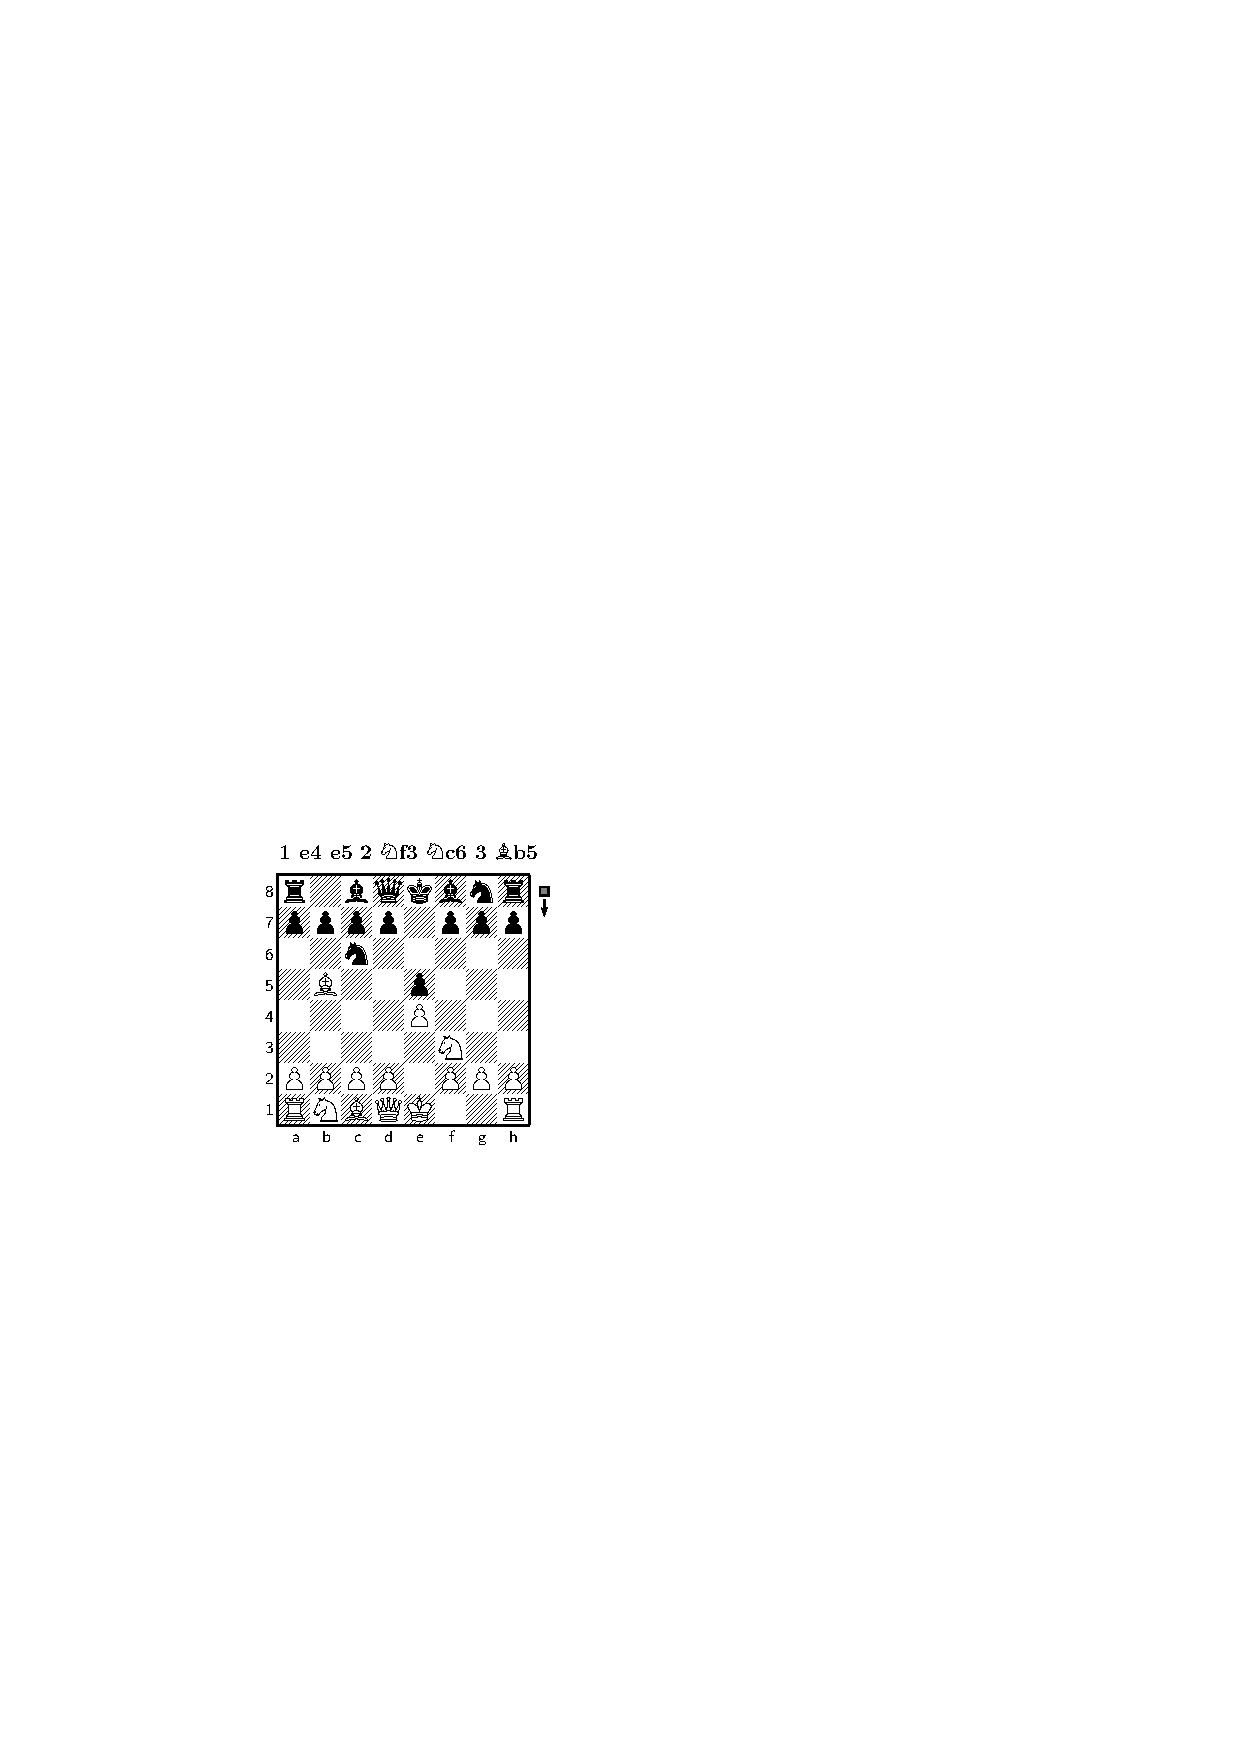
\includegraphics[width=\hsize]{tabuleiro}
    \end{LaTeXoutput}
  \end{column}
\end{columns}
\end{frame}

\begin{frame}{Produzindo partituras musicais com MusiX\TeX}
\begin{itemize}
\item MusiX\TeX{} é incluído no \TeX\ Live;
\item Leia a documentação com o comando \texttt{texdoc musixtex} 
\item Usa notação musical para descrever a partitura;
\item \LCmdArg{usepackage}{musixtex} e \LCmdArg{usepackage}{musixcpt}
\item Rosegarden (sequenciador de midi) -- \url{http://www.rosegardenmusic.com/}
\end{itemize}
\end{frame}

\begin{frame}{Um exemplo de partitura}\fontsize{11}{12}\selectfont
\begin{LaTeXcode}[Fonte da partitura]
\LCmdArg{begin}{music} \string\hsize=100mm \n
\LCmdArg{generalmeter}{\string\meterfrac24}\% \n 
\string\parindent 0pt \string\generalsignature{-3} \n 
\string\startpiece\string\bigaccid \string\NOtes\string\qu\Larg{ce}\string\en\string\bar \n
\string\NOtes\string\qu\Larg{gh}\string\en\string\bar \string\NOtes\string\qu\Larg{=b}\string\en  \n
\string\Notes\string\ds\string\cu g\string\en\string\bar \string\NOtes\string\qu\Larg{\string^f=f}\string\en\string\bar \n
\string\NOtes\string\qu\Larg{=e}\string\itied0e\string\qu\Larg{\string_e}\string\en\string\bar \n
\string\Notes\string\ttie0\string\Qqbu ed\Larg{\string_d}c\string\en\string\bar \n
\string\Notes\string\ibu0b\Larg{-2}\string\qb0\Larg{=b}\string\enotes \n
\string\notes\string\nbbu0\string\qb0\Larg{=a}\string\tqh0N\string\enotes \n
\string\Notes\string\Dqbu cf\string\en\string\bar \n
\string\NOtes\LCmdArg{uptext}{\string\it tr}\string\qu e\%\n
\LCmdArg{uptext}{\string\it tr}\string\qu d\string\en\string\bar \n
\string\NOtes\string\qu c\string\qp\string\en\string\Endpiece \n
\LCmdArg{end}{music} \n
\end{LaTeXcode}
\end{frame}

\begin{frame}{Um exemplo de partitura}
\begin{LaTeXoutput}\centering
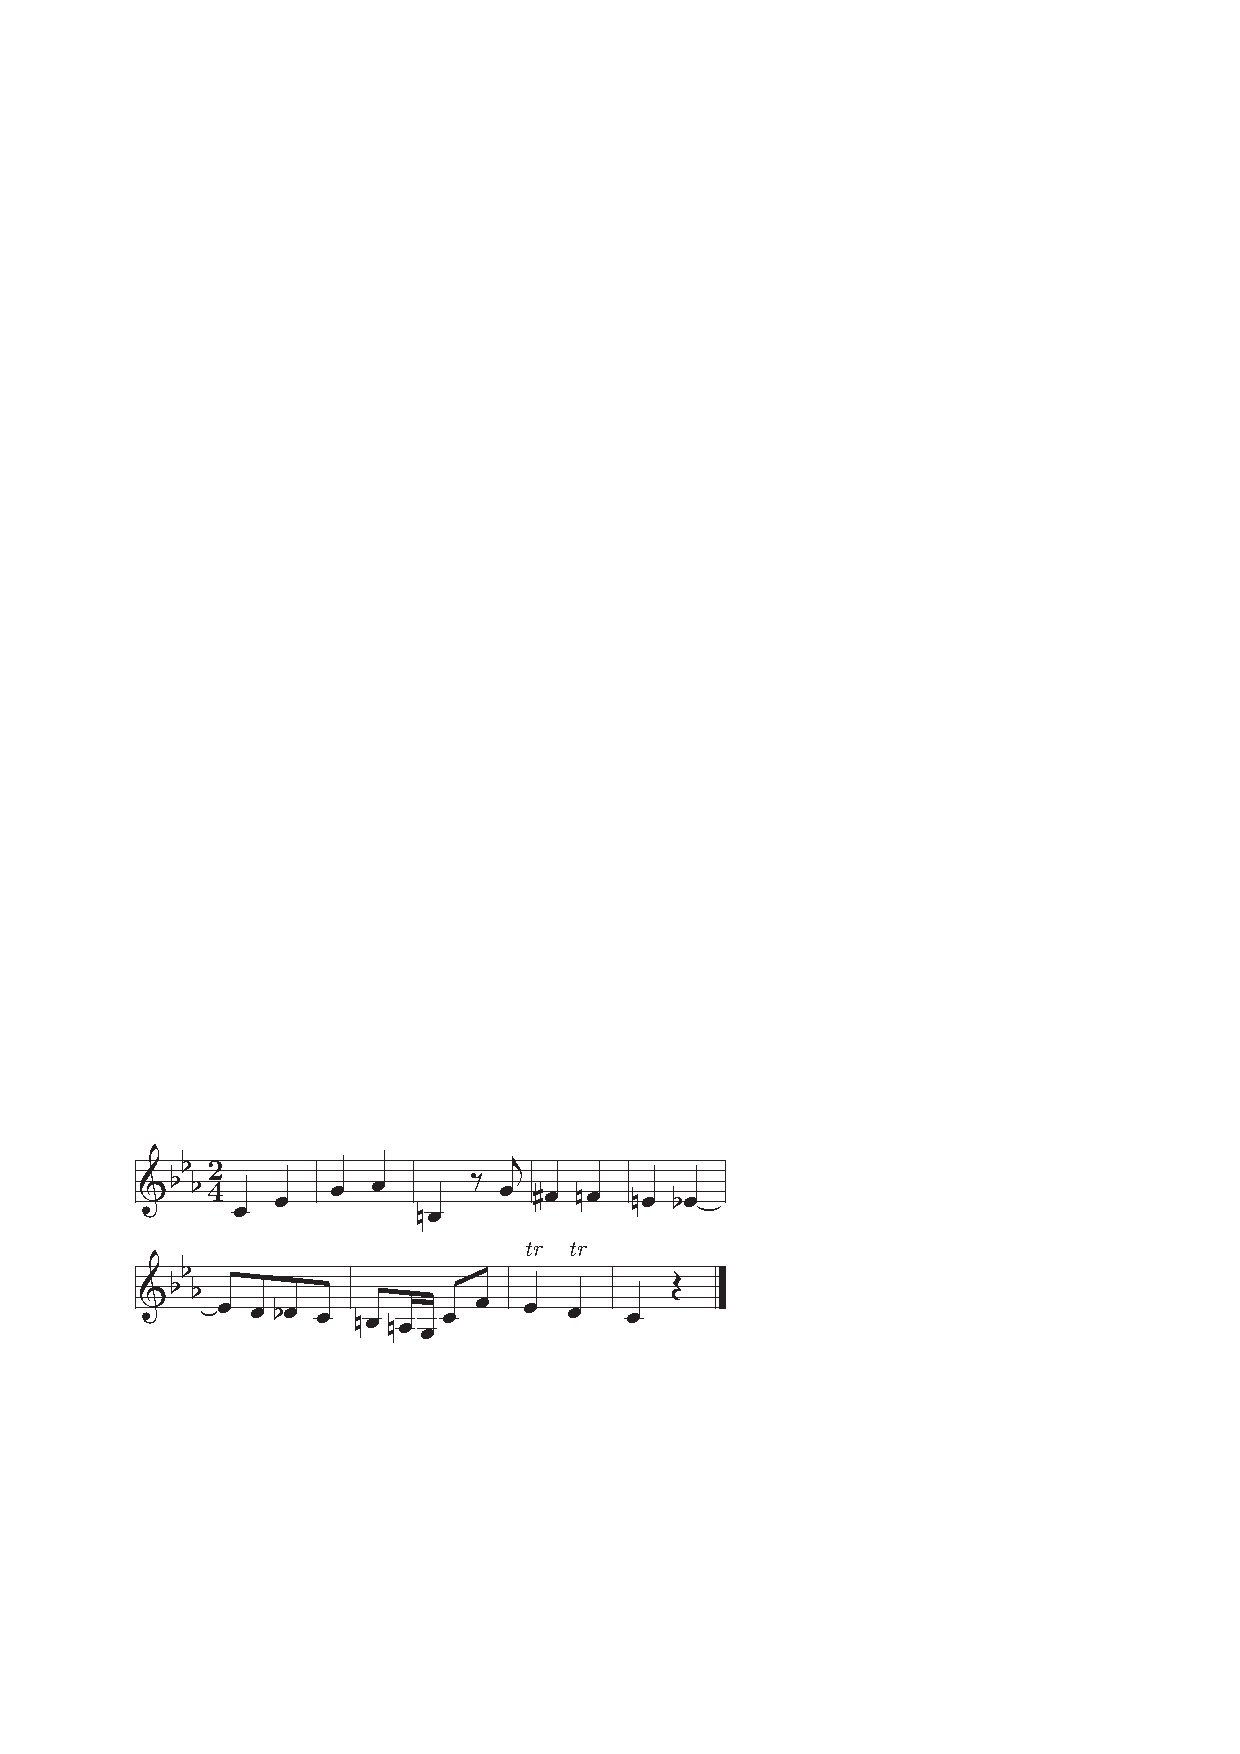
\includegraphics[width=\hsize]{Musica}
\end{LaTeXoutput}

\end{frame}

\begin{frame}[fragile]
\frametitle{Fórmulas químicas}
\begin{itemize}
\item \LaTeX\ possui pacotes para tipografia de textos científicos que, entre outras coisas, permitem a composição de fórmulas químicas;
\item Evita o excesso de subscritos típicos desse tipo de aplicação;
\item Leia a documentação com o comando \texttt{texdoc mhchem};
\item \LCmdOptArg{usepackage}{version=3}{mhchem}
\end{itemize}

\begin{LaTeXcode}[Exemplo]
\LCmdArg{ce}{C6H12O6}
\end{LaTeXcode}

\medskip

Produz:
\begin{LaTeXoutput}
\[ \mathrm{C}_6\mathrm{H}_{12}\mathrm{O}_6 \]
\end{LaTeXoutput}
\end{frame}


